%\chapter{organization}

%%%%%%%%%%%%%%%%%%%%%%%%%%%%%%%%%%%%%%%%%%%%%%
\section{ProtoDUNE-SP organization}

Given its technical challenges, its importance to the DUNE experiment and the timeframe in which it must operate, protoDUNE-SP requires a strong organizational structure with effective leadership to ensure its success. This detector is similar in design to the Short Baseline Neutrino Detector (SBND), the near detector of the SBN experiment at Fermilab. 
\fixme{It may b better to reword this in a less FNAL centric way and emphasize the similarity with the dual phase first, then mention the 
fertile ground that the neutrino platform provides and in that context mention SBND as well.}
The timelines of the two experiments are very similar, and therefore the development of effective synergies, in particular, the exploitation of common detector solutions, common test tooling, and the optimal use of resources (human and financial) will help to achieve the goals of both efforts.  The full description of the protoDUNE-SP organization is in~\cite{pdune-sp-org}.

%%%%%%%%%%%%%%%%%%%%%%%%%
\subsection{A Detector Organization within the DUNE Collaboration}

ProtoDUNE-SP is a detector organization within the DUNE collaboration, at the same level as the Far Detector (FD), Near Detector (ND) and ProtoDUNE-DP organizations, as indicated in Figure~\ref{fig:hi-lev-org-det}. The ProtoDUNE-SP effort is led by three Coordinators, supported by a Deputy, and by a Technical Lead.

\begin{cdrfigure}[High-level organization of the detector efforts within DUNE]{hi-lev-org-det}{High-level organization of the detector efforts within DUNE. Each has a structure of working groups (WG) beneath, dedicated to particular subsystems or components.}
 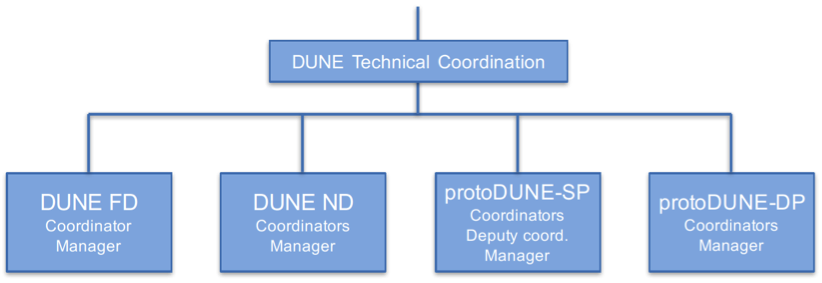
\includegraphics[width=0.95\textwidth]{hi-lev-org-det}
\end{cdrfigure}
%%\fixme{In fig 8.1: DUNE FD coordinator singular?; also I thought we were standardizing on ProtoDUNE not protoDUNE. Anne}

The main ProtoDUNE-SP detector elements (TPC, CE and PDS) are intended as engineering prototypes for the DUNE FD. The DUNE FD organization is responsible for the management of the production of these detector components. The ProtoDUNE-SP organization is responsible for the activities at CERN, including the detector integration, installation, commissioning and operation of the experiment in the charged-particle test beam at the Neutrino Platform.  This also includes interfaces to DUNE Physics and DUNE Computing \& Software organizations. Efficient coordination between the ProtoDUNE-SP and FD organizations is key to success of this project.



Each member of the ProtoDUNE-SP leadership has a distinct role:
\begin{itemize}
\item The DUNE Technical Board (TB), chaired by the DUNE Technical Coordinator, will act as the main decision-making body for the design of the ProtoDUNE-SP detector. All major decisions regarding the design of ProtoDUNE-SP will take place in the TB, which is responsible for the careful evaluation of all technical aspects and prompt selection of available alternatives during the design and construction phases. Both the DUNE FD and the ProtoDUNE-SP leadership are members of the TB, ensuring that all stakeholders are involved in the decision-making process.
\item The ProtoDUNE-SP Coordinators effectively act as spokespersons for the ProtoDUNE-SP project and report to the DUNE management. They are ex-officio members of the DUNE Technical Board (TB).
\item The ProtoDUNE-SP Deputy Coordinator supports the ProtoDUNE-SP coordinators as required and, in addition, oversees the ProtoDUNE-SP scientific activities. 
\item The ProtoDUNE-SP Project Manager is responsible for all project management aspects for ProtoDUNE-SP. He or she maintains and is responsible for the overall schedule for ProtoDUNESP; represents ProtoDUNE-SP in the Far Detector international project management; manages the ProtoDUNE-SP work at CERN and liaises with the CERN teams responsible for the Neutrino Platform infrastructure for installation and operation of ProtoDUNE-SP.
\end{itemize}

%%%%%%%%%%%%%%%%%%%%%%%%%
\subsection{Synergies with ProtoDUNE-DP}

Concurrently with ProtoDUNE-SP, ProtoDUNE-DP will address a complementary part of the DUNE strategy for reaching the design goal of a 40-kt fiducial mass detector. ProtoDUNE-SP and ProtoDUNE-DP share space in the EHN1 experimental hall.  The CERN Neutrino Platform offers great opportunities for utilizing common infrastructures (e.g., the cryogenics system, LAr purification, DAQ, computing) and for an optimal use and sharing of engineering and scientific resources during assembly, commissioning and operation.

As mentioned, ProtoDUNE-SP and ProtoDUNE-DP are placed at the same high level as the far and near detector organizations in the DUNE organizational chart. This fosters a strong coupling and overlap between the two ProtoDUNEs as well as between them and the Far Detector working groups and their activities. It should be noted, however, that the ProtoDUNEs (SP and DP) are identified as distinct organizations that take ownership of and responsibility for their separate experiments.

During a meeting of the two ProtoDUNE management teams at CERN in February 2016, it was agreed that the organizations would pursue common development in several areas either through new joint working groups of the DUNE collaboration or existing working groups, as follows.


\begin{itemize}
\item Online Computing \& Disk Storage -- Joint Working Group
\item Offline Computing -- Common development through DUNE Software \& Computing Working Group
\item Slow Controls -- Joint Working Group
\item DAQ -- Independent efforts but potential for using common software tools
\item High Voltage Delivery -- Joint Working Group
\item Beam Configuration and Instrumentation -- Joint Working Group
\item Field Cage -- Common development through Far Detector CPA/FC/ HV Working Group
\item Beam Window and Plug -- Common development for ProtoDUNEs through Far Detector
\end{itemize}

%%%%%%%%%%%%%%%%%%%%%%%%%
\subsection{Integration with CERN's Neutrino Platform}

As the ProtoDUNE-SP Project Manager is responsible for all project management aspects for ProtoDUNE-SP, he or she is the primary liaison with the CERN teams responsible for the Neutrino Platform infrastructure for installation and operation of ProtoDUNE-SP. \fixme{expect updates here}

%%%%%%%%%%%%%%%%%%%%%%%%%
\subsection{ProtoDUNE-SP Teams and Leadership Responsibilities}

The ProtoDUNE-SP work is divided into several major tasks, each of which has a dedicated team, as illustrated in Figure~\ref{fig:pDUNE-SP-org}.

\begin{cdrfigure}[ProtoDUNE-SP Organization Structure]{pDUNE-SP-org}{ProtoDUNE-SP Organization Structure}
  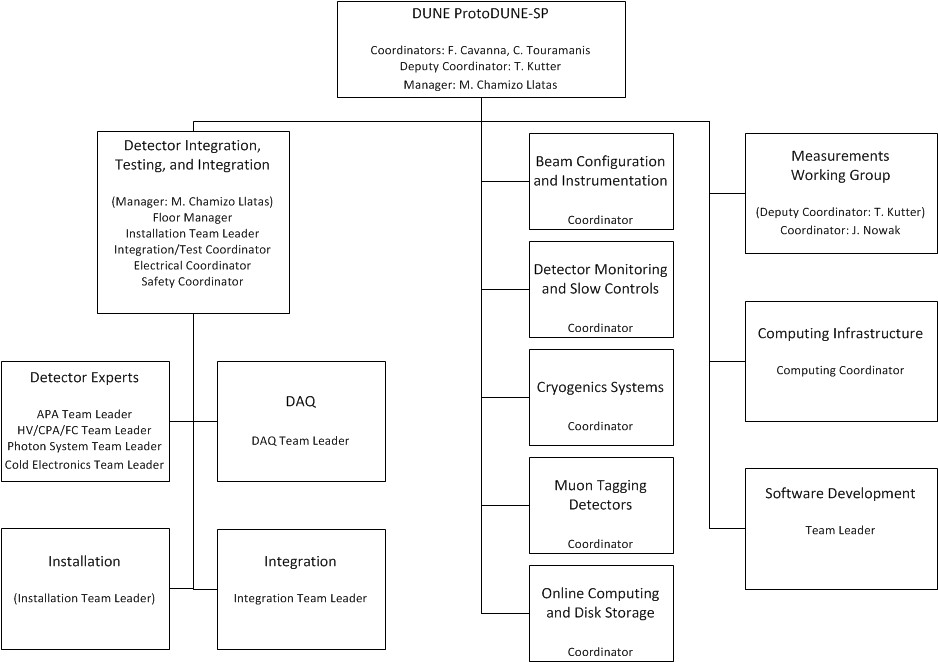
\includegraphics[width=0.95\textwidth]{pDUNE-SP-org.jpeg}
\end{cdrfigure}

\fixme{Find new org chart per Jolie}

%%%%%%%%%%%%
\paragraph{Detector Integration, Testing and Installation (DITI)}

This CERN-based Detector Integration, Testing and Installation (DITI) team is led by a coordinator, with assistance from the installation team leader, other coordinators and Detector Team Leaders.  This team will lead DAQ, installation and engineering integration activities starting from the arrival of the detector components at CERN through to the detector commissioning.

The Technical Lead provides the interface to CERN in all matters related to the infrastructures in the assembly hall and in the experimental hall at the Neutrino Platform, including the cryostat and the cryogenics and LAr purification systems.

Specific team members based at CERN provide the interface between the DITI team and each of the DUNE Far Detector WGs responsible for delivering the ProtoDUNE-SP detector components. 

Correspondingly, the TPC, Photon Detection System and cold electronics WG leaders for the DUNE FD are ex-officio members of the ProtoDUNE-SP DITI managerial structure, ensuring a direct connection. The DITI team includes members (based at CERN) who take responsibility for the major detector components once they are at CERN.

Team leaders for other detector components lead integration, testing and installation work for APA, HV/FC/CPA, photon detector, photon electronics and Cold Electronics.


%%%%%%%%%%%%
\paragraph{High Voltage, Cryogenics, Beam Window and DAQ }

The high voltage (HV) System, Cryogenics System, Beam Window and DAQ are managed by dedicated ProtoDUNE-SP teams. Where appropriate, these teams may overlap with the corresponding ProtoDUNE-DP teams. Team leaders take the responsibility for the timely and technical success of their task. The team leaders will be invited to the DUNE Technical Board meetings when matters relating to ProtoDUNE-SP are discussed.

%%%%%%%%%%%%
\paragraph{Other Tasks}

\begin{itemize}
\item If a Cosmic Muon Tracker/Trigger is implemented for ProtoDUNE-SP, a separate team will be set up mirroring those for the HV and other systems. \fixme{need to clearly state that there will be a muon tagger or scratch this item - NOTE: muon tagger hardware described in section 4}

\item Dedicated ProtoDUNE-SP teams have been set up for the Computing Infrastructure and for Beamline Detectors. They will provide the interface with CERN IT and with the Neutrino Platform and will support the experiment during run operations.
\item The ProtoDUNE-SP physics planning and analysis will be led by Software Development and Physics teams. They will take responsibility for the preparations and fast delivery of detector performance characterization and physics results based on beam and cosmic ray data.
\end{itemize}

%%%%%%%%%%%%%%%%%%%%%%%%%%%%%%%%%%%%%%%%%%%%%%
\subsection{Cost estimate}

%%%%%%%%%%%%
\paragraph{ProtoDUNE-SP costs by subsystem}

The Memorandum of Understanding (MOU) for Collaboration in the Neutrino Program, signed by Sergio Bertolucci and Nigel Lockyer in December 2015 outlined ProtoDUNE-SP CORE costs by subsystem and funding agency.  The CERN Neutrino Platform is providing significant deliverables to enable the successful execution of the DUNE prototyping program, including the experimental hall, beamline, cryostat support structure, and membrane cryostat.  In addition, CERN is providing a significant portion of the cryogenics plant, the cathode plane assemblies, field cage tooling, feedthroughs, DAQ, installation resources, online data processing support, and detector slow controls.  

The costliest element aside from the cryostat and cryogenics, the Anode Plane Assemblies, are being provided by the United States (US-DOE) and the United Kingdom.  The US-DOE is fully funding the Cold Electronics production.  The UK is leading the DAQ system effort, with contributions from the US.  The table shown in Figure~\ref{fig:mou}, from the referenced MOU, outlines the costs and contributing institutions.

\begin{cdrfigure}[Costs and contributing institutions]{mou}{Costs and contributing institutions \fixme{table is outdated as far as institutional responsibilities go - should be updated or a sentence added in text that it has been revised.}}
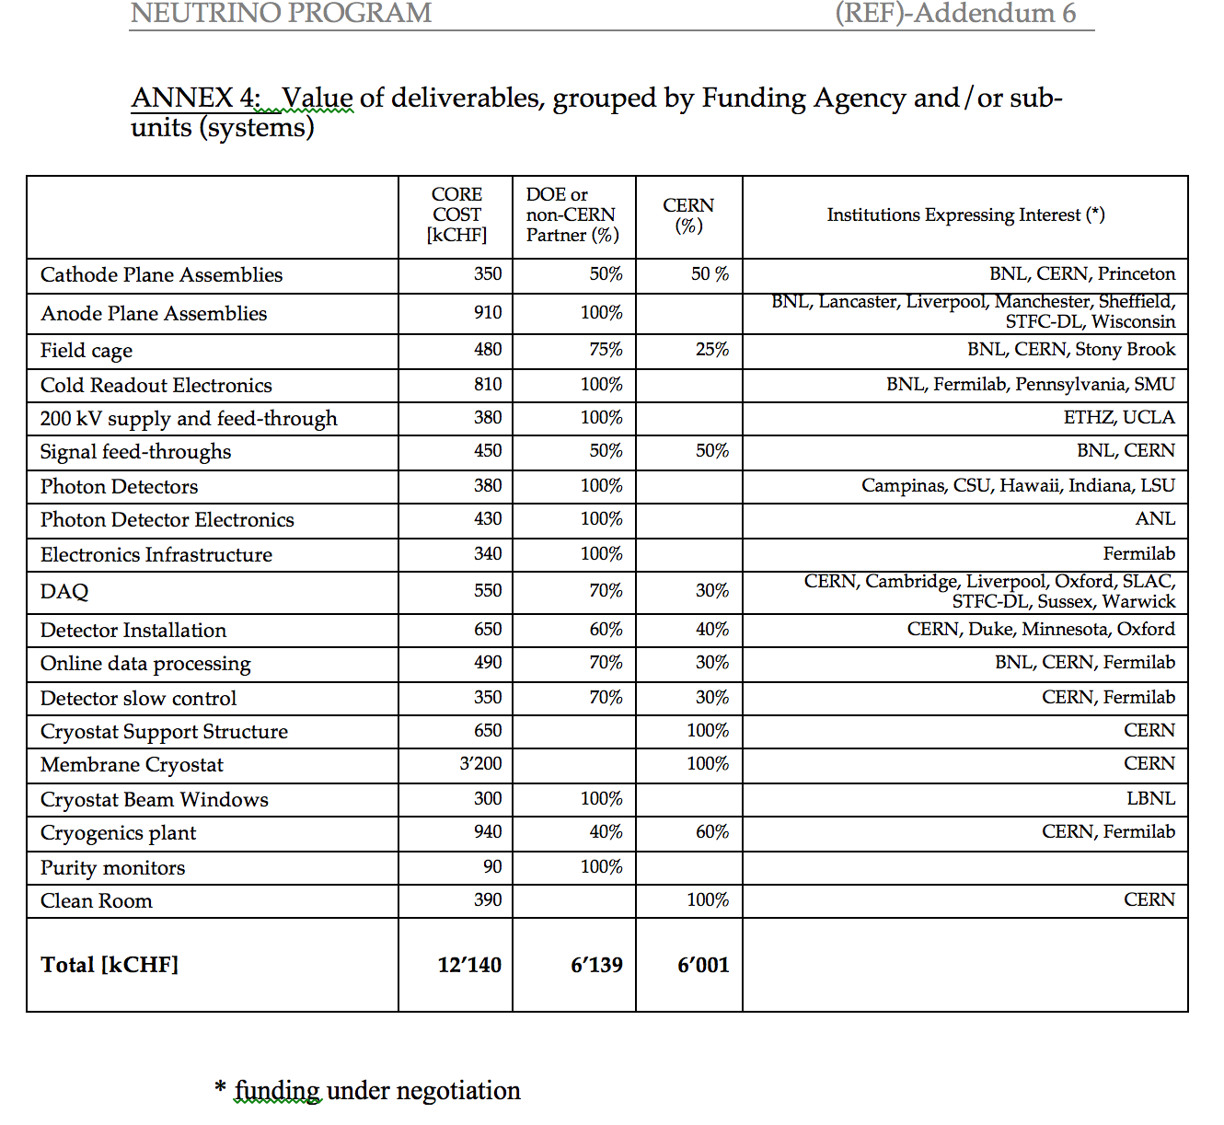
\includegraphics[width=0.8\textwidth]{MOU-picture}
\end{cdrfigure}

%%%%%%%%%%%%
\paragraph{ProtoDUNE-SP operations support}
To enable the success of protoDUNE-SP integration, installation and commissioning activities, the DUNE Collaboration and DUNE Project representatives have requested supplemental funding from the US Department of Energy to support scientist travel to CERN and consumables for the protoDUNE-SP run.  This funding is also intended to support extended scientific personnel stays at CERN for personnel that are not supported by the DUNE project or university research grants. 

In addition, the operations funding request included allocations for consumables such as liquid argon and liquid nitrogen, as well as computing equipment and supplies.  The request is under consideration by US DOE.

%%%%%%%%%%%%%%%%%%%%%%%%%%%%%%%%%%%%%%%%%%%%%%
%\subsection{ProtoDUNE and EHN1 schedule}
\subsection{Schedule}

The schedule summary in Figure~\ref{fig:schedule} outlines the timeline for high-level activities at CERN for ProtoDUNE-SP, including test stands, integration activities, installation and commissioning.  The Detector Integration, Testing and Installation Coordinator, with the system team leaders and the ProtoDUNE-SP Coordinators, is developing a detailed testing protocol and sequencing plan for components.  Detector components will start arriving at CERN in early 2017, and the clean room set up and component testing will start in March 2017. The beam data-taking operation is scheduled to run from the beginning of August 2018 through the end of October 2018.

\begin{cdrfigure}[Schedule summary]{schedule}{Summary of schedule for high-level activities at CERN for ProtoDUNE-SP}
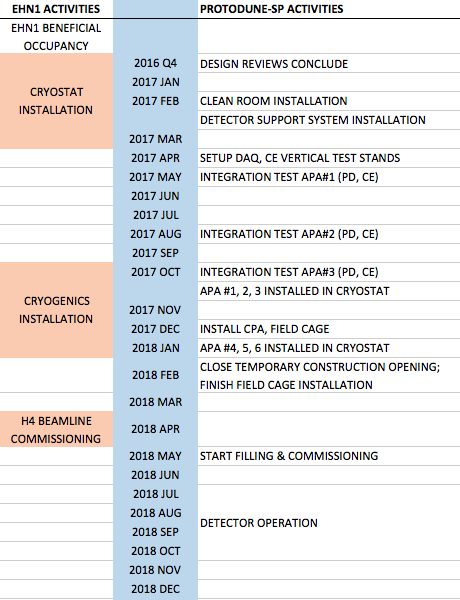
\includegraphics[width=0.95\textwidth]{protodune-sp-schedule-for-tdr}
\end{cdrfigure}